\documentclass[12pt]{article}
\usepackage{graphicx}
\DeclareGraphicsExtensions{.pdf,.png,.jpg}

\title{Scalable\\ Data Integration and Entity Resolution\\in Hadoop}

\author{Eric Peyton\\
\small Georgia Institute of Technology\\
\small CS 4365 Project\\
}

\begin{document}
\maketitle

\begin{abstract}
Data integration is the process of combining multiple data sources through a mapping of schema in order to produce a common unified view of the data. Integrating large datasets introduces a number of new challenges, especially if much of the data is noisy. Entity resolution is the process of resolving duplicated records of entities and relationships between them. This requires some comparison of the records, but can quickly grow inefficient when integrating millions of records from huge datasets. 

I am proposing a Java framework to extend the Apache Hadoop library and facilitate smooth parallel data integration and entity resolution on a cluster. Hadoop provides a powerful platform for parallel computing. However, often many adjustments to an application are required in order to fit the MapReduce programming model. This typically involves much code and testing. For integrating data, this includes writing a custom MapReduce job for every new data source. To resolve entity duplicates, more MapReduce jobs have to written to match, unify, and merge the duplicate entities. The proposed Java framework will greatly simpifly this process and provide tools for integrating large data sources, resolving their records to real-world entities, and exporting the results.
\end{abstract}
\section{Problems Addressed}
In the ``big data'' of today, information about real-world entities often comes from large, diverse, and unstructured sources. \\\\
For example,  we can examine the case of constructing information about real-world events in a city (e.g. a concert, wine-tasting, or festival). 
There is no central or complete source for gathering information about these on-goings. Many are user-submitted through Facebook, others found through ticketing websites, or some may even appear only in the website of a local magazine. 
This data may come in structured or unstructured formats and grows daily among hundreds of cities. 
Since events often appear in multiple sources, the number of event records to organize can easily scale into millions a year. 
The same problem can be extended to different entity types, such as local businesses or human information.\\\\
Scalable techonology is needed to integrate and disambiguate these records into representations of real-world of entities. However, the underlying process for this remains similar across domains and types of entities, such that repetitive work is done for each new entity type. This issue is amplified when a big data platform such as Hadoop requires verbose Java code for MapReduce jobs. A unified and systematic approach to solving the problem would prevent redundant efforts.

\section{Objectives}
In order to address these problems, I created a framework to translate the problems of heterogenous data integration and entity resolution to the MapReduce programming model on the Hadoop platform. \\\\
To limit the scope of the project, I intended to focus on distributed data integration into a record-matching entity resolution framework. 
In my project, resolving entities involves matching them, clustering them on transitive relationships, and computing a single representation of a cluster. 
In addition, this process will be completed with a global schema and schema mappings provided by the user.\\\\
Another objective was to create a generic and unified solution to solve these problems across multiple domains.
In order to accomplish this, I treated the functions for schema-mapping, and matching, and merging as black-box plugins that are provided by a user of the framework. These simple functions help reduce boilerplate code associated with MapReduce jobs and encourage (relatively) concise code to describe the relationships between entities.\\\\
Lastly, this project is intended as a tool for other programmers. 
Implementation of the framework and black-boxes are completely in Java, and there is no GUI component for management by non-technical users. 
This eases integration with Hadoop MapReduce and provides all the logical functionality of Java to users. 

\section{Approach}
This framework is built upon the Hadoop platform and the MapReduce batch-processing programming model. 
Hadoop was chosen for its easy and low-cost scaling abilities, and its popularity among big-data platforms.\\\\
During the researching of this project, I found an excellent paper by Yahoo researchers describing their platform, WOO, that performs what they call ``Knowledge Base Synthesis'' \cite{WOO}.
Their objectives were similar to mine, so I used the paper as a base for this project.\\\\
The data integration and entity resolution process consists of five component jobs: the importers, builder, grouper, combiner, and exporter.
\subsection{Importers}
An importer job is created for each new data source. The framework utilizes both built-in and custom MapReduce input formats for importing data from HDFS into the job. Currently, the project supports JSON, XML, text, and CSV data inputs to an import job. In the importer, each data source is mapped to a global schema using a block-box function that is unique to the data source. Changes in a data source require subsequent changes to its mapping function.\\\\
In the mapper of the importer, an input record is mapped to a serializable Java POJO using automatic and user-provided conversions. These records are then distributed across the cluster to a number of reducers. The reducer machines map the record input schema to the global schema and write the output to an intermediate location on HDFS.\\\\
Additionally, the black-box plugins allow for normalization, validation, and data cleaning during the import stage.
\subsection{Builder}
The builder handles the matching component of the entity resolution process.\\\\
A simple pairwise comparison of every single entity requires $O(n^2)$ comparisons, thus is very inefficient for a large number of records. 
An improvement to pairwise comparison, called ``blocking'', is implemented within the mapper component of the builder.
The entire set of entities to match are distributed into ``blocks'' based on their attributes.
Theoretically, these blocks are computed such that two matching entities are very unlikely to be in the same block.\\\\
For my project, I implemented a simple inverted index blocking function, where entities are blocked by the words in one or more attributes
For instance, when presented with a movie record with the title \textit{Toy Story}, the record is distributed into both the block for \textit{Toy} and the block for \textit{Story}.\\\\
This distribution translates perfectly to MapReduce, where is record is mapped to its blocking words in the mapper. 
In the reducer, every record in each block is compared pairwise using a block-box matching function. 
A utility package provides generic similarity functions to the user, such as Jaccard Similarity and Levenshtein distance. 
The matching pairs are written to another intermediate location on HDFS.
\subsection{Grouper}
The grouper is the only non-MapReduce component of the framework. 
The grouping process involves taking pairs of matching records as input, and transforming these into groups of matching records. 
These groups are created from the understanding of a transitive matching relationship between entities.\\\\
In other terms, if the matching pairs were edges in a graph, then the grouper serves to find all the connected components of the graph.
Because this is essentially a graphing algorithm, it does not translate well to the MapReduce programming model.
Even still, a few projects exist to perform graph processing using MapReduce, such as Apache Giraph \cite{giraph}.\\\\
However, integrating distributed graph processing was beyond the scope of the project. 
Instead, in my framework, I used an iterative algorithm on a single machine.
\subsection{Combiner}
The combiner combines groups of matched entities into a single entity that is representative of the group.
Another black-box user plugin is used for selecting how these entities are combined.
This combination may include a simple union of attributes or more complex logic such as prioritizing entities from higher quality sources.
A mapper-only MapReduce job distributes this work across the cluster of machines.
\subsection{Exporter}
Lastly, the exporter exports the resolved entities. Currently, the exporter is a map-only MapReduce job that exports entities as JSON objects to a folder on HDFS.



\section{Architecture}
\centerline{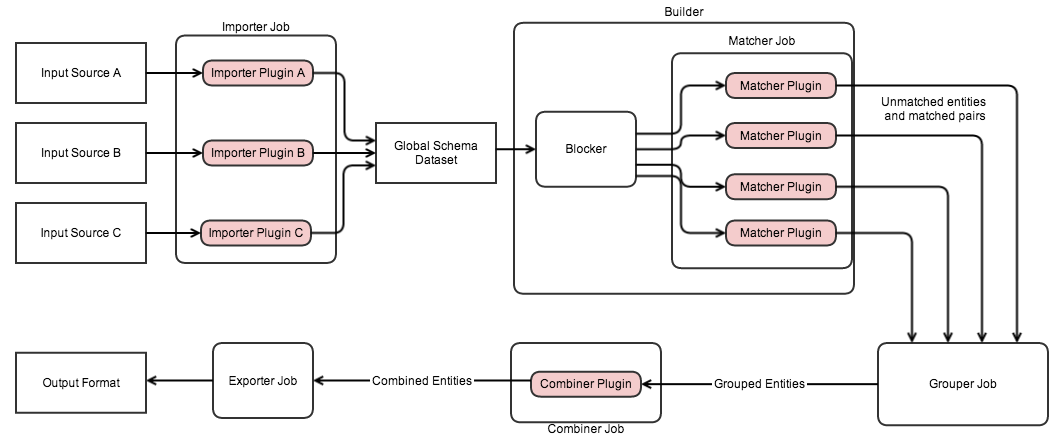
\includegraphics[scale=.5]{architecture}}

\section{Lessons Learned}
Early in the class, we learned about some of challenges of big data, including the challenges of integrating a variety of data sources into to a system. As a result, I adjusted my project to learn both about data integration and entity resolution in a distributed system.
Through this project, I have learned quite a few important lessons. \\\\
First, I realized that not all problems are easily translated to the map reduce programming model.
Graph processing is one of such problems, and is necessary for the entity resolution in the framework I created. This is because the matching is done across multiple machines with no shared resources. As a result, an entity may be detected as a match from different machines, and these transitive relationships must be resolved.\\\\
In addition, I learned that Java generics are not the best solution for creating a unified approach to this framework. 
My platfrom uses generics to manipulate objects during MapReduce and serialize them between jobs.
As a result, I forced to often cast objects in order to pass them around the various components.
In addition, since the framework does not know the global schema itself, it must use reflection to serialize the objects between jobs.\\\\
Lastly, although Java is tightly integrated with the MapReduce framework, it is not ideal language for describing relationships between two entities.
That is, describing complex relationships can quickly become complex when written in Java.
In the future, ontology languages may provide a more fitting solution to this.

\section{Future Work}
There is much improvement that can be done to the framework.\\\\
For example, in the early weeks of class, we learned about quality of information challenge to big data systems. This relates to some of the traditional challenges in entity resolution, such as malformed data. In the future, I would like to focus on creating a more robust framework to handle low quality data in an effective manner.\\\\
Given time, there are quite a few other features I would like to implement:
Blocking methods exist that are proven to be more effective than inverted indexes. One such example is MinHash, which is a type of locality sensitive hashing.
MinHash is able to provide an estimate of the Jaccard index without comparing two sets against each other.\\\\
Utilizing machine learning matching with training sets may provide more accurate matching than simple generic similarity tools.\\\\
Also, implementing the grouping phase as a MapReduce job in Apache Giraph will create a completely distributed process, and eliminate the current bottleneck.\\\\
Currently, the framework is tested with a single limited dataset of products.
Bigger and more diverse data sets may show different results or expose defects.\\\\
Lastly, I would like to utilize languages other than Java for processes like data transformation (such as PigLatin) and ontologies (such as OWL).





\end{document}
